\documentclass{source/Report}

\major{地理信息科学}
\name{陈杰伟}
\title{RV64 内核引导}
\stuid{3200101205}
\college{地球科学学院}
\date{\today}
\lab{玉泉曹光彪-西503}
\course{操作系统}
\instructor{寿黎但}
\grades{}
\expname{RV64 内核引导}
\exptype{编程实验}
\partner{无}

\begin{document}
\makecover
\makeheader
\section{实验目的}
- 学习 RISC-V 汇编, 编写 head.S 实现跳转到内核运行的第一个 C 函数。

- 学习 OpenSBI,理解 OpenSBI 在实验中所起到的作用,并调用 OpenSBI 提供的接口完成字符的输出。

- 学习 Makefile 相关知识, 补充项目中的 Makefile 文件, 来完成对整个工程的管理。

\section{实验环境}
Ubuntu 20.04

\section{实验步骤}
\subsection{编写head.S}

head.S为程序分配程序栈的入口,并且跳转至本程序的入口函数(start\_kernel)

在lds中,链接器已经指明了程序的入口为start标签,kernel代码起始位置为0x80200000。

\begin{lstlisting}[language = c, title = {程序的入口}]
    /* 程序入口 */
    ENTRY( _start )
    
    /* kernel代码起始位置 */
    BASE_ADDR = 0x80200000;
\end{lstlisting}

所以程序开始时,会运行至start标签处,在start标签处编写RISC-V汇编如下,代码意义在注释中说明


\begin{lstlisting}[language = bash, title = {设置栈指针并跳转到主函数}]
    .extern start_kernel #外部引入入口函数start_kernel

    .section .text.entry #指示改部分是text部分的entry
    .globl _start #定义start为全局标签
_start:
    la sp, boot_stack_top #将栈指针寄存器指向栈顶地址
    j start_kernel #跳跃到函数入口的地址
\end{lstlisting}

这段汇编代码使栈指针寄存器指向栈顶,并且跳到入口函数的地址

随后为boot\_stack(即bss部分的stack)分配空间

\begin{lstlisting}[language = bash, title = {分配栈空间}]
    .section .bss.stack
    .globl boot_stack
boot_stack:
    .space 0x4000 #分配栈空间4k

    .globl boot_stack_top
boot_stack_top:
\end{lstlisting}

\subsection{完善 Makefile 脚本}

完善lib文件夹中makefile脚本如下

\begin{lstlisting}[language = bash, title = {makefile}]
    C_SRC       = $(sort $(wildcard *.c)) #获取当前目录所有c文件写入C_SRC变量,wildcard寻找通配符,sort以首字母排序
    OBJ		    = $(patsubst %.c,%.o,$(C_SRC)) #将c文件后缀一一替换成o文件后缀写入OBJ变量
    
    all:$(OBJ) #指定输出目标为OBJ变量文件
    %.o:%.c
        ${GCC} ${CFLAG变量} -c $< #调用GCC编译器编译,中在上一级makefile中GCC编译器写入GCC变量,参数写入CFLAG变量
    clean:
        $(shell rm *.o 2>/dev/null) #使用rm命令进行clean
\end{lstlisting}

编译成功的终端输出如图1

\begin{figure}[p]
    \centering
    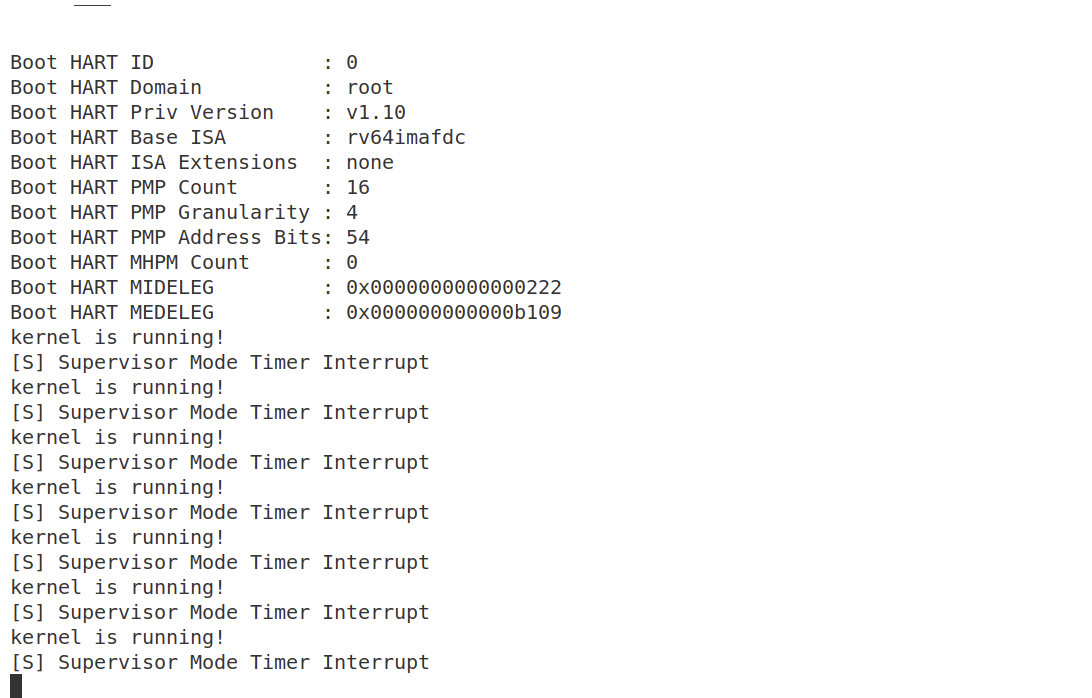
\includegraphics[width = 1\textwidth]{1}
    \caption{编译内核成功}
\end{figure}

输出的vmliunx如图2

\begin{figure}[p]
    \centering
    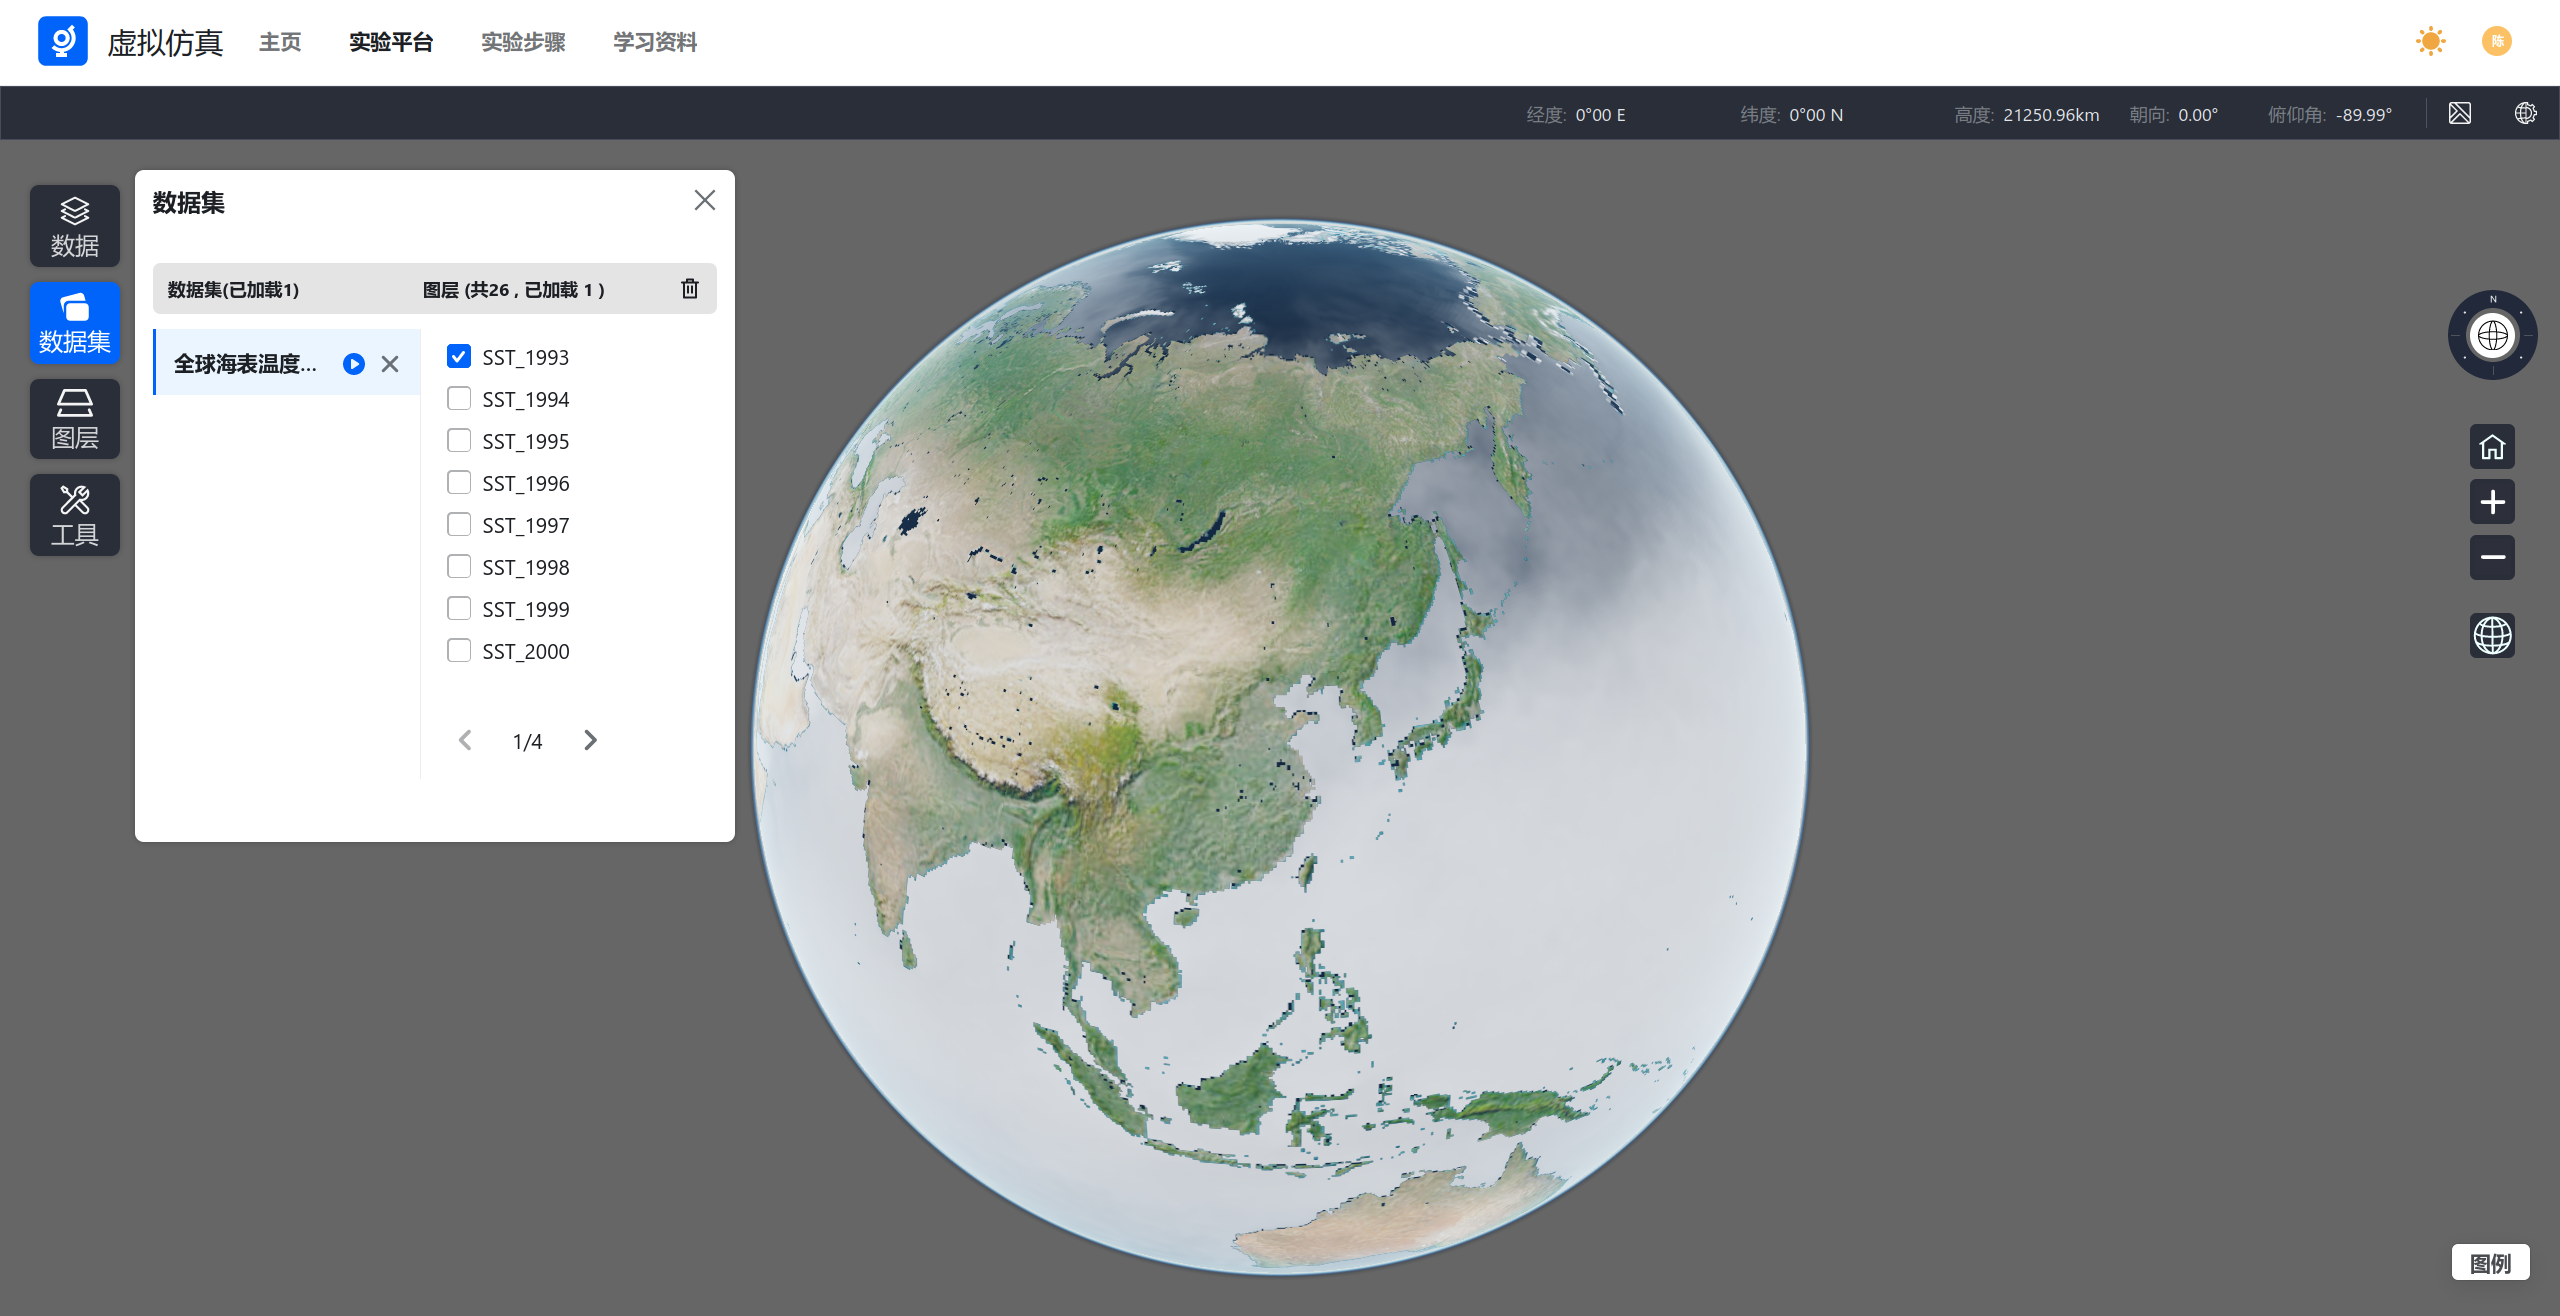
\includegraphics[width = 0.3\textwidth]{2}
    \caption{vmlinux}
\end{figure}

\subsection{补充 sbi.c}

sbi\_ecall 函数的功能是利用ecall指令调用 OpenSBI 接口的功能,实现字符输入输出等功能

1.将 ext (Extension ID) 放入寄存器 a7 中,fid (Function ID) 放入寄存器 a6 中,将 arg0 ~ arg5 放入寄存器 a0 ~ a5 中。

\begin{lstlisting}[language = c, title = {sbi}]
    register unsigned int a0 = 0, a1 = 0;
	__asm__ volatile(
		"mv a7, %[ext]\n"
		"mv a6, %[fid]\n"
		"mv a0, %[arg0]\n"
		"mv a1, %[arg1]\n"
		"mv a2, %[arg2]\n"
		"mv a3, %[arg3]\n"
		"mv a4, %[arg4]\n"
		"mv a5, %[arg5]\n"

		:

		: [ext] "r"(ext),
		  [fid] "r"(fid),
		  [arg0] "r"(arg0),
		  [arg1] "r"(arg1),
		  [arg2] "r"(arg2),
		  [arg3] "r"(arg3),
		  [arg4] "r"(arg4),
		  [arg5] "r"(arg5)

		: "memory");
	//将变量值写入寄存器
\end{lstlisting}

a0-a7是RISC-V标注内专用的保存函数形参的寄存器

2.使用 ecall指令。ecall 之后系统会进入 M 模式,之后 OpenSBI 根据我们传入的参数调用硬件完成相关的指令,然后将返回值存入寄存器a0和a1中,其中 a0 为 error code, a1 为返回值,用 sbiret 来接受这两个返回值作为c的返回值

\begin{lstlisting}[language = c, title = {ecall}]
    __asm__ volatile(
		"ecall" //调用ecall指令

		: [a0] "=r"(a0), [a1] "=r"(a1) //结果写入变量

		:

		: "memory");

	struct sbiret return_value;
	return_value.error = a0;
	return_value.value = a1;

	return return_value;
\end{lstlisting}

在start\_kernel函数中加入

将rootfs copy到Linux源代码根目录,cd到该目录然后执行

\begin{lstlisting}[language = c, title = {测试sbi}]
    sbi_ecall(0x1, 0x0, 0x30, 0, 0, 0, 0, 0) //打印字符0
\end{lstlisting}

并使用make run运行,输出结果如图3

\begin{figure}[p]
    \centering
    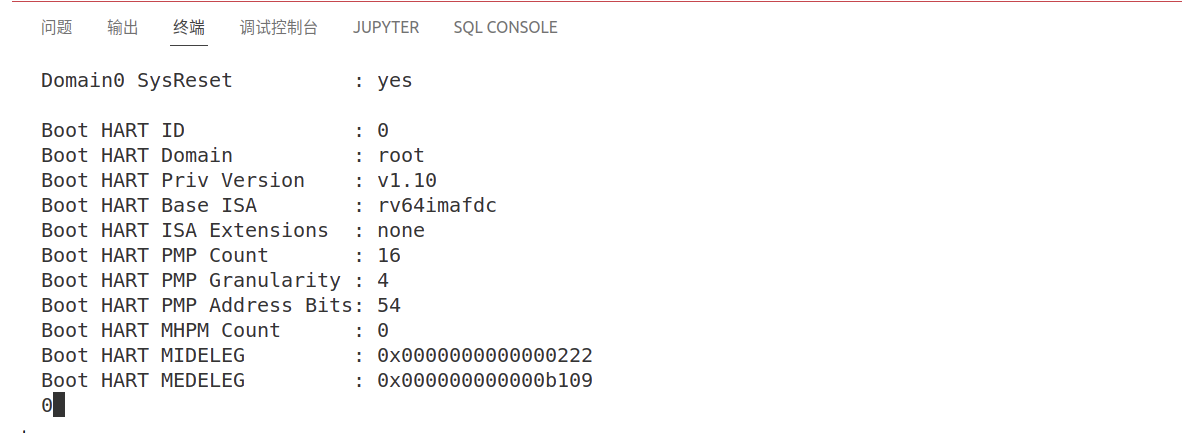
\includegraphics[width = 1\textwidth]{3}
    \caption{sbi运行}
\end{figure}

证明该函数功能正常

\subsection{puts()和 puti()}

puts()函数的实现思路是反复调用sbi打印命令循环打印字符串中每一个字符直到读到0

\begin{lstlisting}[language = c, title = {puts}]
    void puts(char *s) {
        while(*s!='\0')
        {
            uint64 char_code = *s;                        //获取字符编码
            sbi_ecall(0x1, 0x0, char_code, 0, 0, 0, 0, 0);//调用打印字符ecall
            s++;
        }
    
        return;
    }
\end{lstlisting}

puti()的实现思路是将int转化为char*然后调用puts()打印

\begin{lstlisting}[language = c, title = {puti}]
    void puti(int x) {
        char s[int_max] = {0};//分配字符串空间
        int_to_str(x, s);
        puts(s);
    
        return;
    }
\end{lstlisting}

其中int\_to\_str的实现思路是首先读取正负号然后取绝对值,然后从低位到高位逐步写入字符串,然后将字符串数字部分倒转

\begin{lstlisting}[language = c, title = {int转char}]
    void int_to_str(int num, char *str)
    {
        int i = 0;   //指示填充str
        if (num < 0) //如果num为负数,将num变正
        {
            num = -num;
            str[i++] = '-';
        }
        //从低位到高位写入字符串
        do
        {
            str[i++] = num % 10 + code_0;
            num /= 10;                
        } while (num);               
    
        str[i] = '\0';
    
        int j = 0;
        if (str[0] == '-') //如果有负号,负号不用调整
        {
            j = 1; //从第二位开始调整
            ++i;   //由于有负号,所以交换的对称轴也要后移1位
        }
        //将字符串的数字部分倒转
        for (; j < i / 2; j++)
        {
            str[j] = str[j] + str[i - 1 - j];
            str[i - 1 - j] = str[j] - str[i - 1 - j];
            str[j] = str[j] - str[i - 1 - j];
        }
    
        return;
    }
\end{lstlisting}

运行结果如图4

\begin{figure}[p]
    \centering
    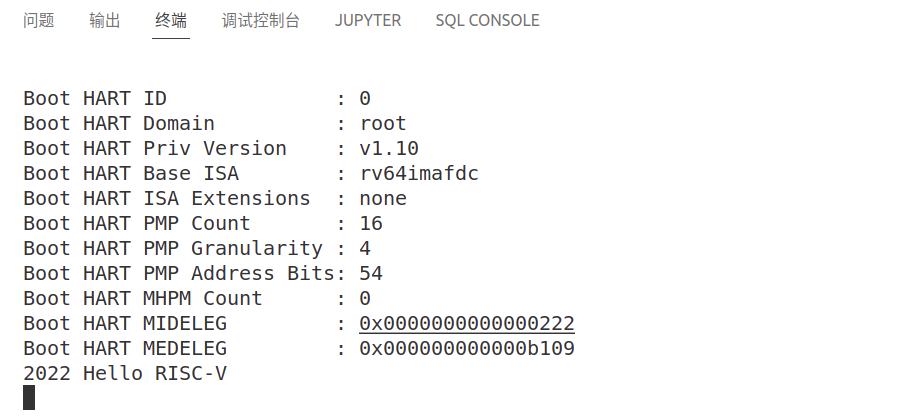
\includegraphics[width = 1\textwidth]{4}
    \caption{打印函数运行结果}
\end{figure}

\subsection{修改 defs}

read\_csr的目的是从指定csr中读取值,具体实现如下

\begin{lstlisting}[language = c, title = {csr宏}]
#define csr_read(csr)                 \
    ({                                \
        register uint64 __v;          \
        asm volatile(                 \
            "csrr %0," #csr           \
            : "=r"(_v)                \
            :                         \
            : "memory");              \
        __v;                          \
    })
\end{lstlisting}

然后在start\_kernel里加入

\begin{lstlisting}[language = c, title = {验证}]
    csr_write(sstatus, 24578);
    puti(csr_read(sstatus));
\end{lstlisting}

运行后读取值如图5

\begin{figure}[p]
    \centering
    
\includegraphics[width = 1\textwidth]{8}
    \caption{读csr}
\end{figure}

写入的值和读取值一致证明csr\_read宏的功能正确

\section{思考题}

1.请总结一下 RISC-V 的 calling convention,并解释 Caller / Callee Saved Register 有什么区别?

RISC-V 的 calling convention简单总结是对RISC-V汇编语言中函数调用的寄存器使用规范,简单总结如图

\begin{figure}[p]
    \centering
    
\includegraphics[width = 1\textwidth]{5}
    \caption{calling convention}
\end{figure}

在编写RISC-V汇编程序时,一定要遵守该寄存器使用方式和命名,这样程序才有足够的共用性,不会产生数据被覆盖的情况。

可以看到寄存器分为两种caller-saved类型和callee-saved类型

caller-saved:可以从该类寄存器中读取数据,写入数据,该寄存器所存储的值在函数调用过程中可能发生改变,比如参数寄存器就属于该类型

callee-saved:该类寄存器中存储的值在函数调用过程中不能改变,比如栈指针寄存器

2.编译之后,通过 System.map 查看 vmlinux.lds 中自定义符号的值(截图)

如图7

\begin{figure}[p]
    \centering
    
\includegraphics[width = 1\textwidth]{6}
    \caption{System.map}
\end{figure}

3.用 csr\_read 宏读取 sstatus 寄存器的值,对照 RISC-V 手册解释其含义(截图)。

将start\_kernel函数改写如下

\begin{lstlisting}[language = c, title = {验证}]
#include "print.h"
#include "sbi.h"
#include "defs.h"
    
    extern void test();
    
    int start_kernel()
    {
    
        puti(2022);
        puts(" Hello RISC-V\n");
    
        puti(csr_read(sstatus));
    
        test(); // DO NOT DELETE !!!
    
        return 0;
    }
\end{lstlisting}

make run运行结果如图8

\begin{figure}[p]
    \centering
    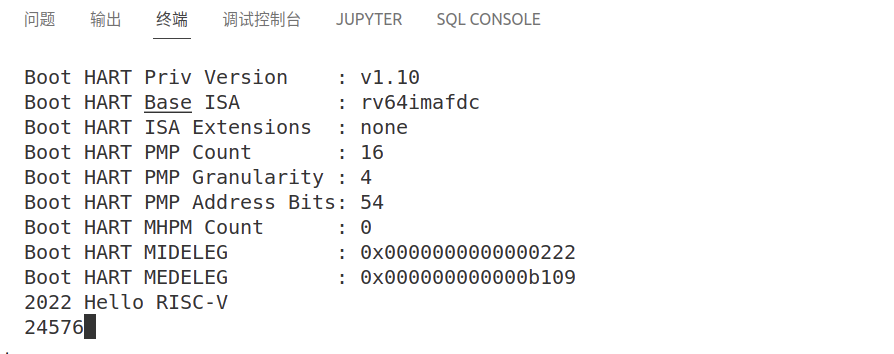
\includegraphics[width = 1\textwidth]{7}
    \caption{读取sstatus}
\end{figure}

状态值24576转化为2进制

0110 0000 0000 0000

翻阅手册获取每一位值的含义如图9

\begin{figure}[p]
    \centering
    
\includegraphics[width = 1\textwidth]{9}
    \caption{sstatus含义}
\end{figure}

SPP 位指示进入管理员模式之前执行的特权级别,当前是0代表用户模式

SIE 位启用或禁用监管者模式下的所有中断,当前是禁用状态

SPIE 位指示在进入管理模式之前是否启用了管理中断。 当前未启用

UIE 位启用或禁用用户模式中断。当前未启用

4.用 csr\_write宏向sscratch寄存器写入数据,并验证是否写入成功(截图)。

编写start\_kernel

\begin{lstlisting}[language = c, title = {验证}]
    int start_kernel()
    {
    
        puti(2022);
        puts(" Hello RISC-V\n");
    
    
        puti(csr_read(sscratch));
        puts("\n");
        csr_write(sscratch, 1);
        puti(csr_read(sscratch));
    
        test(); // DO NOT DELETE !!!
    
        return 0;
    }
\end{lstlisting}

运行结果如图10

\begin{figure}[p]
    \centering
    
\includegraphics[width = 1\textwidth]{10}
    \caption{写入sscratch}
\end{figure}

写入成功

5.Detail your steps about how to get arch/arm64/kernel/sys.i

使用如下bash命令获得编译中间产物sys.i(如图11)

\begin{lstlisting}[language = bash, title = {获取sys.i}]
    make ARCH=arm64 CROSS_COMPILE=aarch64-linux-gnu- defconfig
    make ARCH=arm64 CROSS_COMPILE=aarch64-linux-gnu- arch/arm64/kernel/sys.i
\end{lstlisting}

\begin{figure}[p]
    \centering
    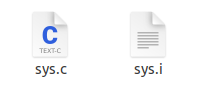
\includegraphics[width = 0.5\textwidth]{11}
    \caption{sys.i}
\end{figure}

6.Find system call table of Linux v6.0 for ARM32, RISC-V(32 bit), RISC-V(64 bit), x86(32 bit), x86\_64 List source code file, the whole system call table with macro expanded, screenshot every step.

利用vscode,查找后缀名为.tbl的文件,如图12

鉴于表太长,我将表的makedown放置在报告的syscall文件夹里

\begin{figure}[p]
    \centering
    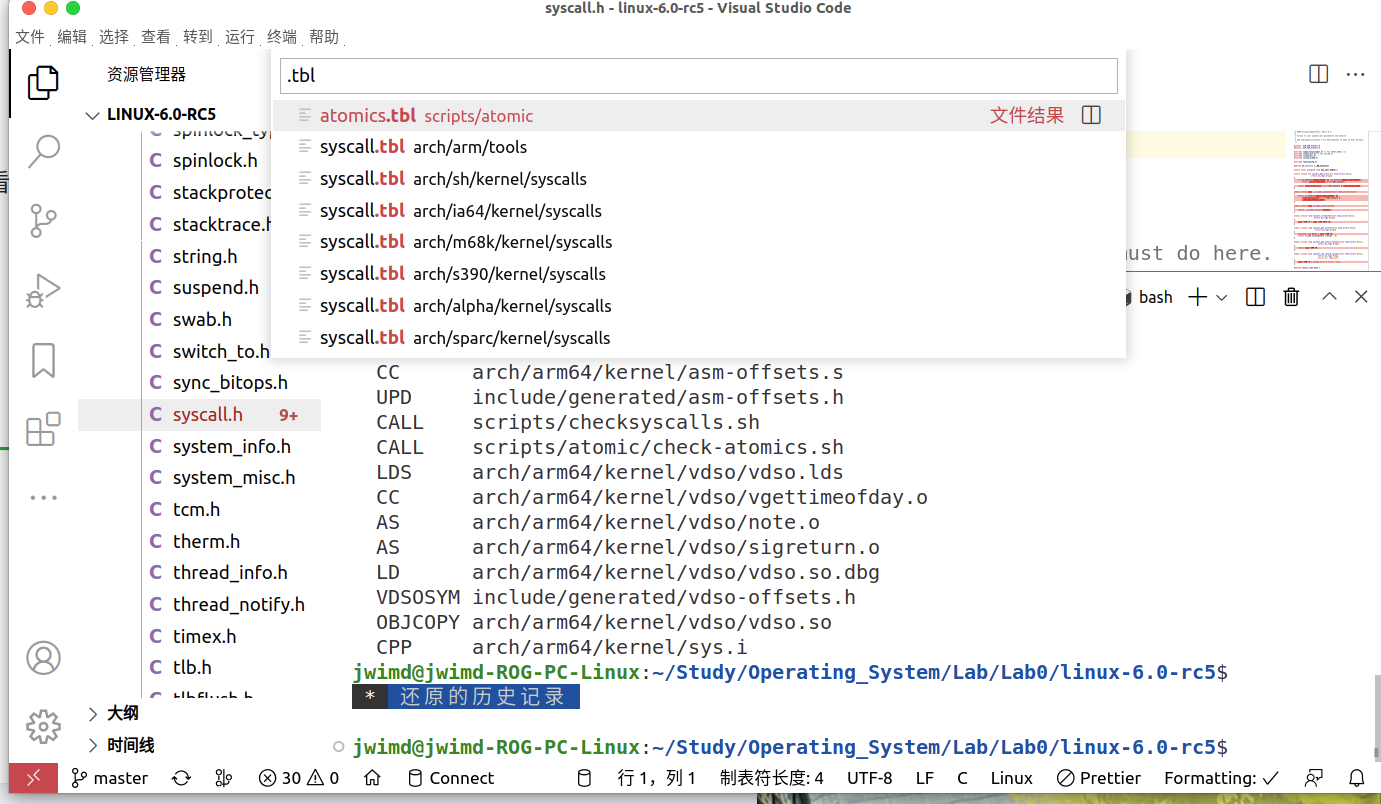
\includegraphics[width = 1\textwidth]{12}
    \caption{vscode查找}
\end{figure}

ARM32: arch/arm/tools/syscall.tbl(见ARM.md)

x86(32 bit):arch/x86/entry/syscalls/syscall\_32.tbl(见x86(32 bit).md)

x86\_64:arch/x86/entry/syscalls/syscall\_64.tbl(见x86\_64.md)

\begin{lstlisting}[language = bash, title = {risc-v获取table}]
    make ARCH=riscv CROSS_COMPILE=riscv64-linux-gnu-arch/riscv/kernel/syscall_table.i #64.bit

    make ARCH=riscv CROSS_COMPILE=riscv32-linux-gnu-arch/riscv/kernel/syscall_table.i #32.bit
\end{lstlisting}

由于RISC-V架构的源文件里没有tbl文件,我通过编译中间产物能够大概获得system\_call\_table,但还没有想出好方法来列表,读取的列表见RISC-V.md

获取sys\_call\_table.i的方法

sys\_call\_table.i附在syscall文件夹内

7.Explain what is ELF file? Try readelf and objdump command on an ELF file, give screenshot of the output. Run an ELF file and cat `/proc/PID /maps` to give its memory layout.

ELF(Executable Linkable Format)是一种 Unix-like系统上的二进制文件格式标准,见图13

\begin{figure}[p]
    \centering
    
\includegraphics[width = 1\textwidth]{17}
    \caption{elf}
\end{figure}

ELF大致分为图14所示的几层

\begin{figure}[p]
    \centering
    
\includegraphics[width = 0.8\textwidth]{13}
    \caption{elf分层}
\end{figure}

我在elf文件夹内编写了一个简单的RISC-V汇编程序,执行寄存器加法

\begin{lstlisting}[language = bash, title = {add}]
	.text			
	.global	_start		

_start:
	li t1, 1		
	li t2, 2		
	add t0, t1, t2	
    

stop:
	j stop			

	.end		
\end{lstlisting}

然后在同一目录下编写makefile文件指定输出为elf。同时指定readelf 和 objdump的伪指令

\begin{lstlisting}[language = bash, title = {makefile}]
    CROSS_COMPILE = riscv64-linux-gnu-
    CFLAGS = -nostdlib
    
    CC = ${CROSS_COMPILE}gcc
    OBJDUMP = ${CROSS_COMPILE}objdump
    READELF = ${CROSS_COMPILE}readelf
    
    EXEC = test
    SRC = ${EXEC}.s
    
    .DEFAULT_GOAL := all
    all:
        @${CC} ${CFLAGS} ${SRC} -o ${EXEC}.elf
    
    .PHONY : objdump
    objdump: all
        @${OBJDUMP} -S ${EXEC}.elf
    
    .PHONY : readelf
    readelf: all
        @${READELF} -S ${EXEC}.elf
    
    .PHONY : clean
    clean:
        rm -rf *.o *.elf	
\end{lstlisting}

执行readelf结果如图15

\begin{figure}[p]
    \centering
    
\includegraphics[width = 0.8\textwidth]{14}
    \caption{readelf结果}
\end{figure}

执行objdump结果如图16

\begin{figure}[p]
    \centering
    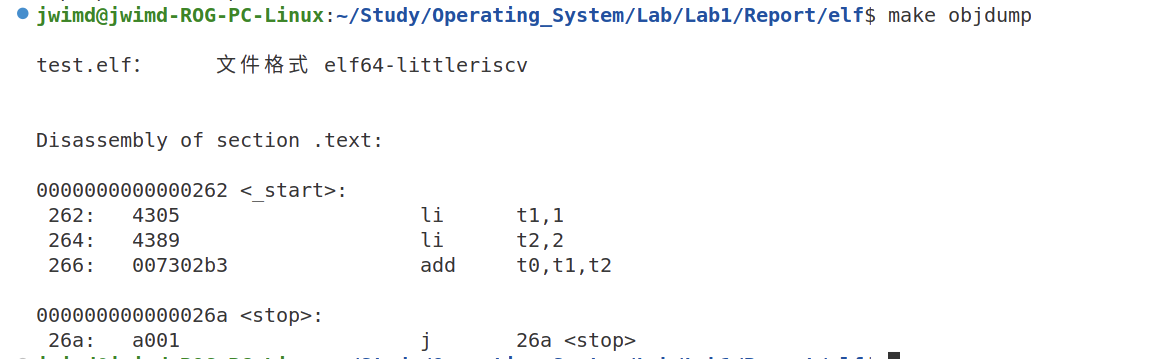
\includegraphics[width = 1\textwidth]{15}
    \caption{objdump结果}
\end{figure}

使用QEMU运行elf,改写makefile

\begin{lstlisting}[language = bash, title = {makefile}]
    CROSS_COMPILE = riscv64-linux-gnu-
    CFLAGS = -nostdlib
    
    CC = ${CROSS_COMPILE}gcc
    OBJDUMP = ${CROSS_COMPILE}objdump
    READELF = ${CROSS_COMPILE}readelf
    
    QEMU = qemu-system-riscv32
    QFLAGS = -nographic -smp 1 -machine virt -bios none
    
    EXEC = test
    SRC = ${EXEC}.s
    
    .DEFAULT_GOAL := all
    all:
        @${CC} ${CFLAGS} ${SRC} -o ${EXEC}.elf
    
    .PHONY : objdump
    objdump: all
        @${OBJDUMP} -S ${EXEC}.elf
    
    .PHONY : run
    run: all
        @${QEMU} ${QFLAGS} -kernel ./${EXEC}.elf
    
    .PHONY : readelf
    readelf: all
        @${READELF} -S ${EXEC}.elf
    
    .PHONY : map
    map: all
        nm ${EXEC}.elf
    
    .PHONY : clean
    clean:
        rm -rf *.o *.elf
\end{lstlisting}

执行make run可以运行一次寄存器加法,可以使用gdb查看

执行make map读取内存结构如图17

\begin{figure}[p]
    \centering
    
\includegraphics[width = 1\textwidth]{16}
    \caption{map}
\end{figure}

\end{document}

